 \documentclass[oneside,12pt]{Classes/UFP}

%% Defina as propriedades do PDF gerado
\ifpdf
    \pdfinfo { /Title  (UFP THESIS)
               /Creator (TeX)
               /Producer (pdfTeX)
               /Author (Christophe Soares csoares@ufp.edu.pt)
               /CreationDate (D:20120101000000)  %format D:YYYYMMDDhhmmss
               /ModDate (D:20121101120000)
               /Subject (Como escrever uma tese em LaTeX)
               /Keywords (PhD, Thesis)}
    \pdfcatalog { /PageMode (/UseOutlines)
                  /OpenAction (fitbh)  }
\fi

% Titulo

\title{Template em \LaTeXe para a \\ [1ex] % espaçamento
	Universidade Fernando Pessoa
}

\ifpdf
  \author{\href{mailto:csoares@ufp.edu.pt}{Christophe Soares}}
  \collegeordept{\href{http://fct.ufp.pt/t}{Faculdade de Ciências e Tecnologia}}
  \university{\href{http://www.ufp.pt}{Universidade Fernando Pessoa}}
% insert below the file name that contains the crest in-place of 'UnivShield'
  \crest{
\includegraphics[width=25mm]{UFP}}
\fi

\degree{Doctor of Philosophy / Master of Science}
\degreedate{2017}

% turn of those nasty overfull and underfull hboxes
\hbadness=10000
\hfuzz=50pt

% Put all the style files you want in the directory StyleFiles and usepackage like this:
\usepackage{StyleFiles/watermark}

% espaçamento de um e meio entre linhas
\onehalfspacing

\begin{document}

% defina a lingua do documento
%\language{english}


% Documento em fase de edição (comentar ou descomentar consoante precisar
\watermark{DRAFT}


\maketitle

%set the number of sectioning levels that get number and appear in the contents
\setcounter{secnumdepth}{3}
\setcounter{tocdepth}{3}

\frontmatter % book mode only
\pagenumbering{roman}

% empty page
\newpage
\thispagestyle{empty}
\mbox{}


% Thesis Abstract -----------------------------------------------------


%\begin{abstractslong}    %uncommenting this line, gives a different abstract heading
\begin{abstracts}        %this creates the heading for the abstract page

Escreva aqui o seu resumo ...

\end{abstracts}
%\end{abstractlongs}



% Thesis Dedictation ---------------------------------------------------

\begin{dedication} %this creates the heading for the dedication page

Coloque aqui a sua dedicatória...

\end{dedication}

% Thesis Acknowledgements ------------------------------------------------


\begin{acknowledgements}      %this creates the heading for the acknowlegments


Gostaria de agradecer...

\end{acknowledgements}




\renewcommand{\contentsname}{{\'I}ndice}
\tableofcontents

\renewcommand{\listfigurename}{{\'I}ndice de Figuras}
\listoffigures

\renewcommand{\listtablename}{{\'I}ndice de Tabelas}
\listoftables

\renewcommand{\nomname}{Nomenclatura}
\printnomenclature  %% Print the nomenclature
\addcontentsline{toc}{chapter}{Nomenclatura}


\renewcommand{\chaptername}{Cap{\'i}tulo}

\mainmatter % book mode only
%%% Thesis Introduction --------------------------------------------------
\chapter{Introdução}
\ifpdf
    \graphicspath{{Introduction/IntroductionFigs/PNG/}{Introduction/IntroductionFigs/PDF/}{Introduction/IntroductionFigs/}}
\else
    \graphicspath{{Introduction/IntroductionFigs/EPS/}{Introduction/IntroductionFigs/}}
\fi

Lorem ipsum dolor sit amet, consectetuer adipiscing elit, sed diam nonummy nibh euismod tincidunt ut laoreet dolore magna aliquam erat volutpat. Ut wisi enim ad minim veniam, quis nostrud exerci tation ullamcorper suscipit lobortis nisl ut aliquip ex ea commodo consequat. Duis autem vel eum iriure dolor in hendrerit in vulputate velit esse molestie consequat, vel illum dolore eu feugiat nulla facilisis at vero eros et accumsan et iusto odio dignissim qui blandit praesent luptatum zzril delenit augue duis dolore te feugait nulla facilisi. Nam liber tempor cum soluta nobis eleifend option congue nihil imperdiet doming id quod mazim placerat facer possim assum. Typi non habent claritatem insitam; est usus legentis in iis qui facit eorum claritatem. Investigationes demonstraverunt lectores legere me lius quod ii legunt saepius. Claritas est etiam processus dynamicus, qui sequitur mutationem consuetudium lectorum. Mirum est notare quam littera gothica, quam nunc putamus parum claram, anteposuerit litterarum formas humanitatis per seacula quarta decima et quinta decima. Eodem modo typi, qui nunc nobis videntur parum clari, fiant sollemnes in futurum.


% \pagebreak[4]
% \hspace*{1cm}
% \pagebreak[4]
% \hspace*{1cm}
% \pagebreak[4]

\chapter{Segundo Capítulo}
\graphicspath{{Chapters/Chapter1/Chapter1Figs/PNG/}{Chapters/Chapter1/Chapter1Figs/PDF/}{Chapters/Chapter1/Chapter1Figs/}}

\section{Primeiro Parágrafo}
Agora começo com o meu primeiro parágrafo aqui... com uma nota de rodapé \footnote{nota de rodapé}.


Segue-se uma equação :
\begin{eqnarray}
CIF: \hspace*{5mm}F_0^j(a) &=& \frac{1}{2\pi \iota} \oint_{\gamma} \frac{F_0^j(z)}{z - a} dz
\end{eqnarray}


\section{Segundo Parágrafo}
e aqui posso escrever mais ... \cite{texbook}

\subsection{Primeiro sub-parágrafo}
... e mais ...
agora posso citar individualmente : \cite{latex} e \cite{texbook}
e \cite{Rud73}; ou agrupando : \cite{latex, texbook, Rud73}.

Vou agora incluir uma imagem :
\begin{figure}[!htbp]
  \begin{center}
    \leavevmode
    \ifpdf
      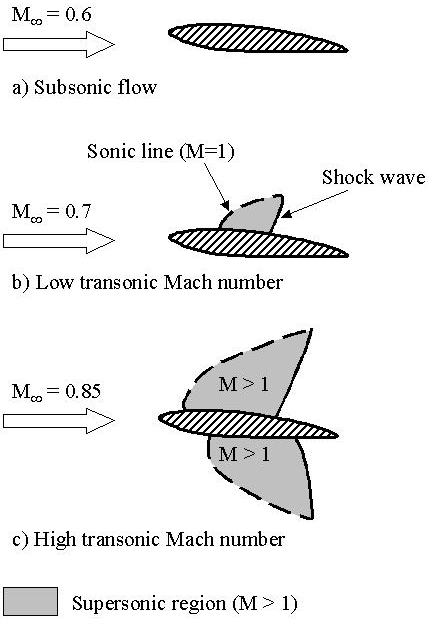
\includegraphics[height=6in]{aflow}
    \fi
    \caption{Legenda}
    \label{FigAir}
  \end{center}
\end{figure}

Posso colocar uma referência cruzada no texto desta forma (\ref{FigAir}) e esta referência cruzada encontra-se na página \pageref{FigAir}. 


\chapter{Terceiro Capítulo}

\graphicspath{{Chapters/Chapter2/Chapter2Figs/PNG/}{Chapters/Chapter2/Chapter2Figs/PDF/}{Chapters/Chapter2/Chapter2Figs/}}

\section{Primeiro Parágrafo}
Segue-se uma tabela:
\begin{table}[tbh!]
\caption{Tabela} 
\label{tab:demo-1}
\centering
\begin{tabular}{l*{6}{c}r}
\hline
Team              & P & W & D & L & F  & A & Pts \\
\hline
FC Porto & 6 & 4 & 0 & 2 & 10 & 5 & 12  \\
Celtic            & 6 & 3 & 0 & 3 &  8 & 9 &  9  \\
FC Copenhagen           & 6 & 2 & 1 & 3 &  7 & 8 &  7  \\
SL Benfica     & 6 & 2 & 1 & 3 &  5 & 8 &  7  \\
\end{tabular}
\end{table}

\chapter{Quarto Capítulo}

\graphicspath{{Chapters/Chapter3/Chapter3Figs/PNG/}{Chapters/Chapter3/Chapter3Figs/PDF/}{Chapters/Chapter3/Chapter3Figs/}}


\section{Primeiro Parágrafo}

Segue-se mais uma equação:
\begin{equation}
a=\frac{N}{A}
\end{equation}%

\nomenclature{$a$}{The number of angels per unit area}%
\nomenclature{$N$}{The number of angels per needle point}%
\nomenclature{$A$}{The area of the needle point}%

The equation $\sigma = m a$%
\nomenclature{$\sigma$}{The total mass of angels per unit area}%
\nomenclature{$m$}{The mass of one angel}
follows easily.

\def\baselinestretch{1}
\chapter{Conclusões}

\graphicspath{{Chapters/Conclusions/ConclusionsFigs/PNG/}{Chapters/Conclusions/ConclusionsFigs/PDF/}{Chapters/Conclusions/ConclusionsFigs/}}



Segue-se as minhas conclusões...

\backmatter % book mode only
\appendix
\chapter{Annexo A}

Lorem ipsum dolor sit amet, consectetuer adipiscing elit, sed diam nonummy nibh euismod tincidunt ut laoreet dolore magna aliquam erat volutpat. Ut wisi enim ad minim veniam, quis nostrud exerci tation ullamcorper suscipit lobortis nisl ut aliquip ex ea commodo consequat. Duis autem vel eum iriure dolor in hendrerit in vulputate velit esse molestie consequat, vel illum dolore eu feugiat nulla facilisis at vero eros et accumsan et iusto odio dignissim qui blandit praesent luptatum zzril delenit augue duis dolore te feugait nulla facilisi. Nam liber tempor cum soluta nobis eleifend option congue nihil imperdiet doming id quod mazim placerat facer possim assum. Typi non habent claritatem insitam; est usus legentis in iis qui facit eorum claritatem. Investigationes demonstraverunt lectores legere me lius quod ii legunt saepius. Claritas est etiam processus dynamicus, qui sequitur mutationem consuetudium lectorum. Mirum est notare quam littera gothica, quam nunc putamus parum claram, anteposuerit litterarum formas humanitatis per seacula quarta decima et quinta decima. Eodem modo typi, qui nunc nobis videntur parum clari, fiant sollemnes in futurum.



%escolha um dos 3 estilos de bibliografia
\bibliographystyle{plainnat}

\renewcommand{\bibname}{Referências Bibliográficas}
\bibliography{References/references} 		% Caminho para o bibtex

\end{document}
